% specification
% run the program

\section{Following paths}

\paragraph{Follow the carrot}{
    There are several ways to make a robot following a trajectory. For the
assignment, as it is suggested, I decided to implement the algorithm
\textit{follow the carrot}. This simple algorithm is presented by Barton in
his PhD thesis\cite{thesis:barton}. The figure \ref{algo:base} takes over
this method.
}

\begin{figure}[!h]
    \begin{algorithmic}
        \ForAll{point in path}
            \State $position \gets \Call{getRobotRosition}$
            \While{$position \neq point$}
                \State $speeds \gets \Call{compute\_speeds(position, point)}$
                \State $setSpeeds( speeds )$
                \State $position \gets \Call{getRobotRosition}$
            \EndWhile
        \EndFor
    \end{algorithmic}
    
    \caption{
        \label{algo:base}
        \textit{Follow the carrot} algorithm
    }
\end{figure}

\paragraph{Speeds computation}{
    The functions called in this algorithm already exists and are designed to
control or to get the robot position. But there no way to compute the speeds, so
I implemented the function \texttt{compute\_speeds} which computes the angular 
and the linear speed of the robot regarding his position and the target position.
This function is presented figure \ref{algo:speeds}. It is essentially about
using mathematical functions and it works.
}

\begin{figure}[!h]
    \begin{algorithmic}
     \Function{compute\_speeds}{robot, carrot}
        \State $distance \gets \sqrt{(carrot.x - robot.x)^{2} + (carrot.y - robot.y)^{2}}$
        \State $robot\_angle \gets \Call{getRobotSteering}$
        \State $carrot\_angle \gets atan2(carrot.y - robot.x, carrot.x - robot.x)$
        \State $angle = carrot\_angle - robot\_angle$
        \State $angular\_speed = angle / 1$
        \State $linear\_speed \gets angular\_speed \times \frac{distance}{2 \times sin( angle )} $
        \State \Return $linear\_speed,~angular\_speed$
     \EndFunction
    \end{algorithmic}
    
    \caption{
        \label{algo:speeds}
        Algorithm to compute the speed to reach a target point
    }
\end{figure}

\begin{figure}[!h]
    \begin{center}
        % Graphic for TeX using PGF
% Title: /home/ens15/ens15bsf/edu/5dv121/lab1/report/src/figures/long_path.dia
% Creator: Dia v0.97.3
% CreationDate: Tue Oct 27 16:01:42 2015
% For: ens15bsf
% \usepackage{tikz}
% The following commands are not supported in PSTricks at present
% We define them conditionally, so when they are implemented,
% this pgf file will use them.
\ifx\du\undefined
  \newlength{\du}
\fi
\setlength{\du}{15\unitlength}
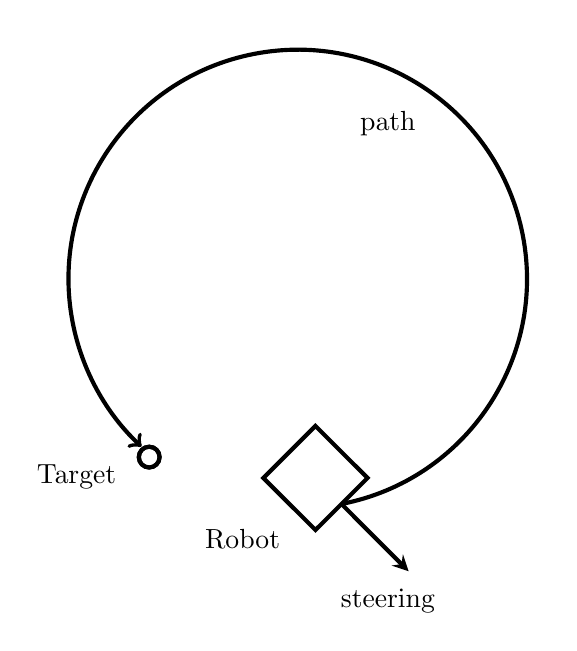
\begin{tikzpicture}
\pgftransformxscale{1.000000}
\pgftransformyscale{-1.000000}
\definecolor{dialinecolor}{rgb}{0.000000, 0.000000, 0.000000}
\pgfsetstrokecolor{dialinecolor}
\definecolor{dialinecolor}{rgb}{1.000000, 1.000000, 1.000000}
\pgfsetfillcolor{dialinecolor}
\pgfsetlinewidth{0.100000\du}
\pgfsetdash{}{0pt}
\pgfsetdash{}{0pt}
\pgfsetbuttcap
{
\definecolor{dialinecolor}{rgb}{0.000000, 0.000000, 0.000000}
\pgfsetfillcolor{dialinecolor}
% was here!!!
\pgfsetarrowsend{stealth}
\definecolor{dialinecolor}{rgb}{0.000000, 0.000000, 0.000000}
\pgfsetstrokecolor{dialinecolor}
\draw (40.907057\du,26.405166\du)--(42.500000\du,28.000000\du);
}
\pgfsetlinewidth{0.100000\du}
\pgfsetdash{}{0pt}
\pgfsetdash{}{0pt}
\pgfsetmiterjoin
\definecolor{dialinecolor}{rgb}{0.000000, 0.000000, 0.000000}
\pgfsetstrokecolor{dialinecolor}
\draw (40.255330\du,24.500000\du)--(41.510660\du,25.752665\du)--(40.255330\du,27.005330\du)--(39.000000\du,25.752665\du)--cycle;
% setfont left to latex
\definecolor{dialinecolor}{rgb}{0.000000, 0.000000, 0.000000}
\pgfsetstrokecolor{dialinecolor}
\node at (40.255330\du,25.947665\du){};
\pgfsetlinewidth{0.100000\du}
\pgfsetdash{}{0pt}
\pgfsetdash{}{0pt}
\pgfsetbuttcap
\pgfsetmiterjoin
\pgfsetlinewidth{0.100000\du}
\pgfsetbuttcap
\pgfsetmiterjoin
\pgfsetdash{}{0pt}
\definecolor{dialinecolor}{rgb}{1.000000, 1.000000, 1.000000}
\pgfsetfillcolor{dialinecolor}
\pgfpathellipse{\pgfpoint{36.250000\du}{25.250000\du}}{\pgfpoint{0.250000\du}{0\du}}{\pgfpoint{0\du}{0.250000\du}}
\pgfusepath{fill}
\definecolor{dialinecolor}{rgb}{0.000000, 0.000000, 0.000000}
\pgfsetstrokecolor{dialinecolor}
\pgfpathellipse{\pgfpoint{36.250000\du}{25.250000\du}}{\pgfpoint{0.250000\du}{0\du}}{\pgfpoint{0\du}{0.250000\du}}
\pgfusepath{stroke}
\pgfsetbuttcap
\pgfsetmiterjoin
\pgfsetdash{}{0pt}
\definecolor{dialinecolor}{rgb}{0.000000, 0.000000, 0.000000}
\pgfsetstrokecolor{dialinecolor}
\pgfpathellipse{\pgfpoint{36.250000\du}{25.250000\du}}{\pgfpoint{0.250000\du}{0\du}}{\pgfpoint{0\du}{0.250000\du}}
\pgfusepath{stroke}
\pgfsetlinewidth{0.100000\du}
\pgfsetdash{}{0pt}
\pgfsetdash{}{0pt}
\pgfsetbuttcap
{
\definecolor{dialinecolor}{rgb}{0.000000, 0.000000, 0.000000}
\pgfsetfillcolor{dialinecolor}
% was here!!!
\pgfsetarrowsend{to}
\definecolor{dialinecolor}{rgb}{0.000000, 0.000000, 0.000000}
\pgfsetstrokecolor{dialinecolor}
\pgfpathmoveto{\pgfpoint{40.882550\du}{26.379091\du}}
\pgfpatharc{79}{-227}{5.522390\du and 5.522390\du}
\pgfusepath{stroke}
}
% setfont left to latex
\definecolor{dialinecolor}{rgb}{0.000000, 0.000000, 0.000000}
\pgfsetstrokecolor{dialinecolor}
\node at (38.500000\du,27.222500\du){Robot};
% setfont left to latex
\definecolor{dialinecolor}{rgb}{0.000000, 0.000000, 0.000000}
\pgfsetstrokecolor{dialinecolor}
\node at (34.500000\du,25.722500\du){Target};
% setfont left to latex
\definecolor{dialinecolor}{rgb}{0.000000, 0.000000, 0.000000}
\pgfsetstrokecolor{dialinecolor}
\node at (42.000000\du,17.222500\du){path};
% setfont left to latex
\definecolor{dialinecolor}{rgb}{0.000000, 0.000000, 0.000000}
\pgfsetstrokecolor{dialinecolor}
\node at (42.000000\du,28.722500\du){steering};
\end{tikzpicture}

    \end{center}
    
    \caption{
        \label{fig:path}
        Path used to reach the target
    }
\end{figure}

\paragraph{}{
    In fact, the way I compute the speeds, and in particular the angular speed can be improved. Let's say the schema at figure \ref{fig:path} represents what the robot currently do. The straight arrow representes the steering of the robot, and the other one stqnds for the trajectory the follows currently. As you can notice it could be quicker ans smart to turn to the other way. To do, when I compute the angle between the robot and the carrot, I just have to check if the angle is lower than $-\pi$ or if it is greater than $\pi$, if so, I add\/substract in the first case $2\pi$. That turns the algoirthms to the one at figure \ref{algo:speeds_smart}.
}

\begin{figure}[!h]
    \begin{algorithmic}
     \Function{compute\_speeds}{robot, carrot}
        \State $distance \gets \sqrt{(carrot.x - robot.x)^{2} + (carrot.y - robot.y)^{2}}$
        \State $robot\_angle \gets \Call{getRobotSteering}$
        \State $carrot\_angle \gets atan2(carrot.y - robot.x, carrot.x - robot.x)$
        \State $angle = carrot\_angle - robot\_angle$
        \If{ $-\pi > angle$ }
            \State $ angle \gets 2\pi + angle $
        \EndIf
        \If{ $\pi < angle$ }
            \State $ angle \gets 2\pi - angle $
        \EndIf
        \State $angular\_speed = angle / 1$
        \State $linear\_speed \gets angular\_speed \times \frac{distance}{2 \times sin( angle )} $
        \State \Return $linear\_speed,~angular\_speed$
     \EndFunction
    \end{algorithmic}
    
    \caption{
        \label{algo:speeds_smart}
        Algorithm to compute the speed to reach a target point
    }
\end{figure}

\paragraph{}{
}

\paragraph{}{
    To makes the robot following the path, I decided to implement the
algorithm called \textit{Follow the carrot}\cite{thesis:barton}. His name is
due to the way it processes the path points. Each point are considered. 
For each point the algorithm computes the angle to turn to reach the carrot
point and the distance between the robot and the carrot point. Once the
angle and the distance are computed, I can compute a linear and an angular
speed to move the robot. The algorithm is very simple but is not efficient.
In fact, many points can be skipped. So in order to improve the robot speed,
the first step was to skip some point by adding a look-ahead distance to the
algorithm. Rather than trying to reach each point, the robot tries to reach
the next carrot point in the look-ahead distance.
}

\paragraph{}{
    The next improvement made was to change how the algorithm used the
points. The first version considers every point (or at least the ones in the
look-ahead distance) and wait one second before considering the next points.
But the this amount of time is totally arbitrary. So, to be more precis and
don't wait too much time or too less time, the algorithm waits till the robot
reach the point before considering the next one:
}

% improv
